\section{Marco Teórico}

\subsection{Contratación pública, corrupción y riesgo}

La contratación pública es el mecanismo mediante el cual el Estado transforma recursos fiscales en bienes, servicios y obras para la ciudadanía. En Colombia, su marco normativo (Ley 80 de 1993 y Ley 1150 de 2007) enfatiza transparencia, selección objetiva y eficiencia, pero la literatura evidencia que, aun con reglas formales, persisten vulnerabilidades institucionales y operativas \cite{mendieta2022regimen, sierra2025contratacion}.

En ese contexto, el riesgo en contratación no debe entenderse únicamente como ``acto corrupto probado'', sino como la probabilidad de desviaciones relevantes en costo, plazo o calidad asociadas a patrones de comportamiento observables en los datos contractuales \cite{salazar2024vigia, calderon2025contratacion}. Esta perspectiva es consistente con enfoques de supervisión preventiva: en lugar de esperar sanciones ex post, se prioriza la detección temprana de contratos con mayor probabilidad de incumplimiento o irregularidad.

La evidencia internacional y regional describe mecanismos recurrentes de afectación del proceso competitivo: colusión entre oferentes, coordinación de precios, rotación de ganadores, direccionamiento de requisitos y fragmentación estratégica de procesos \cite{decarolis2022corruption, spagnolo2024bidrigging, zhang2022collusion}. Todos estos fenómenos reducen la presión competitiva y generan sobrecostos, por lo que son conceptualmente relevantes para este anteproyecto, cuyo problema central es identificar de forma anticipada contratos con señales de alerta en bases como SECOP.

Un aporte clave de la literatura aplicada al sector público es diferenciar \textit{desperdicio activo} (conductas deliberadas para capturar rentas) y \textit{desperdicio pasivo} (ineficiencias por limitaciones técnicas, organizacionales o de diseño institucional) \cite{salazar2024vigia}. Esta distinción justifica el enfoque del estudio: el modelo no pretende ``probar delito'', sino clasificar riesgo operativo y de integridad para apoyar priorización de control.

\subsection{Detección de corrupción y colusión basada en datos}

La detección basada en datos parte del supuesto de que los procesos de contratación dejan huellas estructuradas. Dado que los procedimientos se repiten en el tiempo y comparten campos administrativos comparables, es posible extraer patrones de comportamiento y convertirlos en variables analíticas \cite{zhang2022collusion, tas2024machine}. En la literatura, estas variables operan como \textit{red flags} y permiten estimar riesgo de manera escalable \cite{decarolis2022corruption, lyra2022fraud}.

Entre las señales más reportadas se encuentran: concentración de adjudicaciones en pocos proveedores, dispersión inusual de descuentos, secuencias repetitivas de participación entre los mismos oferentes y variaciones atípicas entre monto adjudicado, tiempo de ejecución y modificaciones contractuales \cite{decarolis2022corruption, wachs2019network}. En términos teóricos, estas señales no se interpretan de forma aislada; su valor explicativo emerge cuando se analizan de manera conjunta.

Para este anteproyecto, la implicación es directa: el problema de investigación se traduce en un flujo de analítica de riesgo donde los datos administrativos se transforman en variables predictoras y, posteriormente, en un puntaje o clase de riesgo para priorizar supervisión.

\begin{figure}[H]
    \centering
    \shorthandoff{<>}
    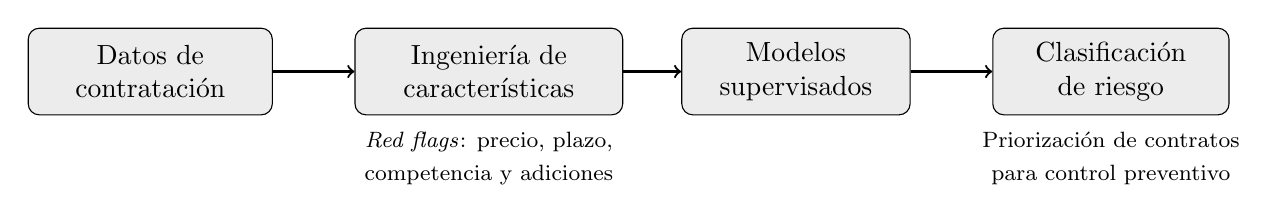
\begin{tikzpicture}[x=1cm,y=1cm]
        \node[draw, rounded corners, fill=gray!15, align=center, minimum width=3.1cm, minimum height=1.1cm] (a) at (0,0) {Datos de\\contratación};
        \node[draw, rounded corners, fill=gray!15, align=center, minimum width=3.4cm, minimum height=1.1cm] (b) at (4.3,0) {Ingeniería de\\características};
        \node[draw, rounded corners, fill=gray!15, align=center, minimum width=2.9cm, minimum height=1.1cm] (c) at (8.2,0) {Modelos\\supervisados};
        \node[draw, rounded corners, fill=gray!15, align=center, minimum width=3.0cm, minimum height=1.1cm] (d) at (12.2,0) {Clasificación\\de riesgo};

        \draw[->, thick] (a) -- (b);
        \draw[->, thick] (b) -- (c);
        \draw[->, thick] (c) -- (d);

        \node[align=center] at (4.3,-1.1) {\footnotesize \textit{Red flags}: precio, plazo,\\ \footnotesize competencia y adiciones};
        \node[align=center] at (12.2,-1.1) {\footnotesize Priorización de contratos\\ \footnotesize para control preventivo};
    \end{tikzpicture}
    \shorthandon{<>}
    \caption{Esquema conceptual del enfoque de detección de riesgo en contratación pública.}
    \label{fig:flujo-riesgo-contratacion}
\end{figure}

Como se observa en la Figura~\ref{fig:flujo-riesgo-contratacion}, la contribución teórica del estudio consiste en conectar la literatura de \textit{red flags} y colusión con un esquema operativo de clasificación de contratos, orientado a apoyar decisiones de vigilancia y no a sustituir el análisis jurídico posterior.

\subsection{Aprendizaje automático para la predicción de riesgos}

El aprendizaje automático supervisado permite estimar una función $f(\mathbf{x})$ que aproxima la relación entre un conjunto de variables contractuales $\mathbf{x}$ y una etiqueta de riesgo $y$ derivada de evidencia histórica \cite{tas2024machine, gallego2021preventing}. En términos aplicados, esta formulación es pertinente para el anteproyecto porque permite pasar de descripciones agregadas a predicciones a nivel de contrato.

Los algoritmos considerados son:

\begin{enumerate}
        \item \textbf{Regresión Logística.} Modela la probabilidad condicional de riesgo como:
        \[
            \hat{p}(y=1\mid \mathbf{x}) = \sigma\!\left(\beta_0 + \sum_{j=1}^{p} \beta_j x_j\right),
            \qquad \sigma(z)=\frac{1}{1+e^{-z}}.
        \]
        Aquí, $x_j$ representa la $j$-ésima variable del contrato (por ejemplo, modalidad, número de oferentes o historial de adiciones), y $\beta_j$ cuantifica su contribución marginal sobre el logaritmo de las probabilidades. Se usa como línea base por su interpretabilidad y trazabilidad para auditoría \cite{gallego2021preventing}.

        \item \textbf{Random Forest.} Combina $T$ árboles de decisión y obtiene la clase final por voto mayoritario:
        \[
            \hat{y} = \operatorname{mode}\left(h_1(\mathbf{x}), h_2(\mathbf{x}), \ldots, h_T(\mathbf{x})\right).
        \]
        Cada árbol captura interacciones no lineales; el ensamble reduce varianza y mejora estabilidad predictiva frente a ruido en los datos administrativos \cite{decarolis2022corruption, salazar2024vigia}.

        \item \textbf{XGBoost.} Construye un ensamble aditivo de árboles, donde la predicción se expresa como:
        \[
            \hat{y}_i = \sum_{k=1}^{K} f_k(\mathbf{x}_i), \qquad f_k \in \mathcal{F}.
        \]
        El entrenamiento minimiza una pérdida con regularización:
        \[
            \mathcal{L} = \sum_{i} l(y_i,\hat{y}_i) + \sum_{k}\Omega(f_k).
        \]
        En esta formulación, $l(\cdot)$ mide el error predictivo y $\Omega(\cdot)$ penaliza complejidad del modelo para controlar sobreajuste. Esta propiedad resulta útil en datos de contratación con alta heterogeneidad \cite{alshboul2022extreme, tas2024machine}.
\end{enumerate}

La selección de estos tres modelos responde a un criterio metodológico complementario: interpretabilidad (Regresión Logística), robustez no lineal (Random Forest) y capacidad predictiva de frontera (XGBoost), en línea con aplicaciones recientes en analítica de contratación \cite{salazar2024vigia, gallego2021preventing}.

\subsection{Evaluación de modelos y construcción de la variable objetivo}

La evaluación en problemas de riesgo contractual exige métricas sensibles al desbalance de clases. Si los contratos de alto riesgo son minoría, la exactitud global puede ser alta aun con desempeño deficiente en la clase crítica. Por ello se priorizan precisión, \textit{recall}, F1 y AUC-ROC \cite{salazar2024vigia, tas2024machine}. Sea $TP$ verdaderos positivos, $FP$ falsos positivos, $TN$ verdaderos negativos y $FN$ falsos negativos:

\begin{figure}[H]
    \centering
    \shorthandoff{<>}
    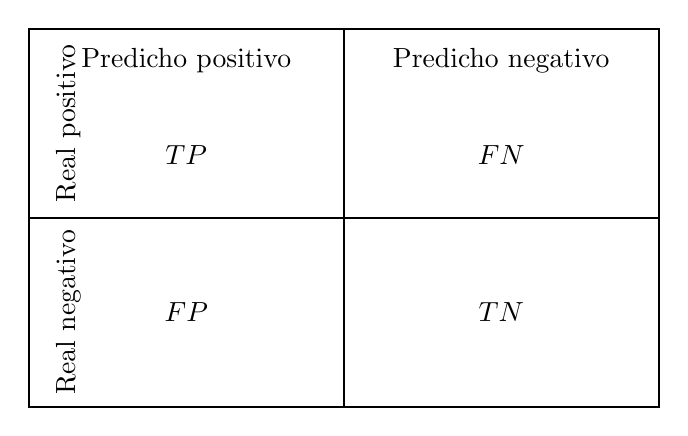
\begin{tikzpicture}[x=1cm,y=1cm]
        \draw[thick] (0,0) rectangle (8,4.8);
        \draw[thick] (0,2.4) -- (8,2.4);
        \draw[thick] (4,0) -- (4,4.8);
        \node at (2,4.4) {Predicho positivo};
        \node at (6,4.4) {Predicho negativo};
        \node[rotate=90] at (0.5,3.6) {Real positivo};
        \node[rotate=90] at (0.5,1.2) {Real negativo};
        \node at (2,3.2) {$TP$};
        \node at (6,3.2) {$FN$};
        \node at (2,1.2) {$FP$};
        \node at (6,1.2) {$TN$};
    \end{tikzpicture}
    \shorthandon{<>}
    \caption{Matriz de confusión para clasificación binaria de riesgo contractual.}
    \label{fig:matriz-confusion-riesgo}
\end{figure}

La Figura~\ref{fig:matriz-confusion-riesgo} muestra que cada métrica enfatiza un tipo de error distinto. En contratación pública, perder casos riesgosos ($FN$) puede ser más costoso institucionalmente que revisar casos adicionales ($FP$), por lo que la interpretación de métricas debe alinearse con el objetivo de vigilancia preventiva.

La \textit{precisión} mide qué proporción de contratos clasificados como riesgosos realmente lo son:

\[
\text{Precisión} = \frac{TP}{TP + FP}
\]

El \textit{recall} (sensibilidad) mide cuántos contratos riesgosos reales logra detectar el modelo:

\[
\text{Recall} = \frac{TP}{TP + FN}
\]

El \textit{F1-score} resume el balance entre precisión y \textit{recall}:

\[
F1 = 2 \cdot \frac{\text{Precisión} \cdot \text{Recall}}{\text{Precisión} + \text{Recall}}
\]

equivalentemente,

\[
F1 = \frac{2TP}{2TP + FP + FN}
\]

La curva ROC compara capacidad de detección y tasa de falsas alarmas a distintos umbrales:

\[
\text{TPR} = \frac{TP}{TP + FN}, \qquad
\text{FPR} = \frac{FP}{FP + TN}
\]

El \textit{AUC-ROC} es el área bajo la curva ROC; valores cercanos a 1 implican mejor poder discriminativo y valores cercanos a 0.5 equivalen a un clasificador aleatorio:

\[
AUC = \int_0^1 \text{TPR}( \text{FPR}) \, d(\text{FPR})
\]

Para robustecer la estimación se emplea validación cruzada estratificada con $k=5$, manteniendo la proporción de clases en cada pliegue y reduciendo sesgo por particiones favorables \cite{tas2024machine, gallego2021preventing}.

Debido a que las bases administrativas no incluyen una etiqueta jurídica explícita de ``corrupción'', la variable objetivo se construye con \textit{proxies} de riesgo de incumplimiento o anomalía operacional, en línea con la literatura aplicada \cite{gomez2025data, gomez2025analyzing, dulce2021deteccion}. A nivel formal, para cada contrato $i$:

\[
y_i =
\begin{cases}
1, & \parbox[t]{0.72\linewidth}{si presenta al menos una señal proxy de riesgo (adiciones reiteradas, suspensiones o desviaciones relevantes en tiempo/costo)} \\
0, & \text{en caso contrario}
\end{cases}
\]

Esta definición no reemplaza el juicio legal ni la auditoría sustantiva, pero sí permite construir un sistema de alerta temprana técnicamente justificable para priorizar revisión institucional.